\apendice{Documentación de usuario}

\section{Requisitos software y hardware para ejecutar el proyecto.}
%Añadir requisitos y tablas de requisitos, pensar si se quieren dividir en requisitos funcionales y no funcionales.
\subsection{Requisitos funcionales}

%%%%%%%%%%%%%%%%%%%%%%%%%%%%% RF-01 %%%%%%%%%%%%%%%%%%%%%%%%%%%%
\begin{table}[h!]
\begin{tabular}{|
>{\columncolor[HTML]{EFEFEF}}c |l|}
\hline
\cellcolor[HTML]{B9E3F0}\textbf{RF-01} & \multicolumn{1}{c|}{\cellcolor[HTML]{B9E3F0}\textbf{Aplicación}}                                                                                                                                                                                \\ \hline
Descripción                            & \begin{tabular}{p{10.5cm}}La solución deberá contar con una aplicación, ya sea una aplicación de escritorio, web o móvil, para simplificar la experiencia de uso y la visualización de resultados por parte del usuario.\end{tabular} \\ \hline
Importancia                            & \cellcolor[HTML]{FFFFFF}\begin{tabular}{p{10.5cm}}Alta, es la base de la visualización del seguimiento de la persona que utiliza el dispositivo.\end{tabular}                                                                               \\ \hline
Prioridad                              & \multicolumn{1}{c|}{Alta}                                                                                                                                                                                                                       \\ \hline
\end{tabular}
\caption{Requisito Funcional 1 'Aplicación'}
\label{RF_01}
\end{table}

%%%%%%%%%%%%%%%%%%%%%%%%%%%%% RF-02 %%%%%%%%%%%%%%%%%%%%%%%%%%%%
\begin{table}[h!]
\begin{tabular}{|
>{\columncolor[HTML]{EFEFEF}}c |l|}
\hline
\cellcolor[HTML]{B9E3F0}\textbf{RF-02} & \multicolumn{1}{c|}{\cellcolor[HTML]{B9E3F0}\textbf{Iniciar grabación}}                                                                                                                                                                                \\ \hline
Descripción                            & \begin{tabular}{p{10.5cm}}La solución deberá contar con una opción de grabación, con la cual el profesional o el usuario tendrán la posibilidad de comenzar y finalizar el registro de la postura.\\ Los resultados durante la grabación se almacenarán en la plataforma para su análisis.\end{tabular} \\ \hline
Importancia                            & \cellcolor[HTML]{FFFFFF}\begin{tabular}{p{10.5cm}}Alta, ya que la grabación de las respuestas permitirá al profesional analizarlas de forma detallada con el objetivo de obtener conclusiones y determinar el grado y evolución de la afectación.\end{tabular}                                                                               \\ \hline
Prioridad                              & \multicolumn{1}{c|}{Alta}                                                                                                                                                                                                                       \\ \hline
\end{tabular}
\caption{Requisito Funcional 2 'Iniciar grabación'}
\label{RF_02}
\end{table}

%%%%%%%%%%%%%%%%%%%%%%%%%%%%% RF-03 %%%%%%%%%%%%%%%%%%%%%%%%%%%%
\begin{table}[h!]
\begin{tabular}{|
>{\columncolor[HTML]{EFEFEF}}c |l|}
\hline
\cellcolor[HTML]{B9E3F0}\textbf{RF-03} & \multicolumn{1}{c|}{\cellcolor[HTML]{B9E3F0}\textbf{Identificación de perfiles}}                                                                                                                                                                                \\ \hline
Descripción                            & \begin{tabular}{p{10.5cm}}La aplicación debe ser capaz de diferenciar a diferentes perfiles, en el caso de uso de una organización o un profesional, y una única identificación en el caso de que se trate de un usuario particular.\end{tabular} \\ \hline
Importancia                            & \cellcolor[HTML]{FFFFFF}\begin{tabular}{p{10.5cm}}Media, una vez se obtenga la base del dispositivo y su funcionamiento se puede dividir a los usuarios entre profesionales o particulares, con distintas funciones para cada uno de ellos.\end{tabular}                                                                               \\ \hline
Prioridad                              & \multicolumn{1}{c|}{Media}                                                                                                                                                                                                                       \\ \hline
\end{tabular}
\caption{Requisito Funcional 3 'Identificación de perfiles'}
\label{RF_03}
\end{table}

%%%%%%%%%%%%%%%%%%%%%%%%%%%%% RF-04 %%%%%%%%%%%%%%%%%%%%%%%%%%%%
\begin{table}[h!]
\begin{tabular}{|
>{\columncolor[HTML]{EFEFEF}}c |l|}
\hline
\cellcolor[HTML]{B9E3F0}\textbf{RF-04} & \multicolumn{1}{c|}{\cellcolor[HTML]{B9E3F0}\textbf{Detección de la postura}}                                                                                                                                                                                \\ \hline
Descripción                            & \begin{tabular}{p{10.5cm}}La solución deberá ser capaz de detectar los cambios en la postura. Para ello se deberá implementar un algoritmo que filtre en función de los datos en crudo recogidos, una postura correcta o incorrecta. Esta medición se podría obtener en forma de ‘porcentaje de buena postura’.\end{tabular} \\ \hline
Importancia                            & \cellcolor[HTML]{FFFFFF}\begin{tabular}{p{10.5cm}}Alta, dado que es la base que permitirá definir si la persona lleva una buena postura o no, y en base a ello, realizar la comunicación correspondiente y obtener las estadísticas necesarias para la toma de decisiones.\end{tabular}                                                                               \\ \hline
Prioridad                              & \multicolumn{1}{c|}{Alta}                                                                                                                                                                                                                       \\ \hline
\end{tabular}
\caption{Requisito Funcional 4 'Detección postural'}
\label{RF_04}
\end{table}

%%%%%%%%%%%%%%%%%%%%%%%%%%%%% RF-05 %%%%%%%%%%%%%%%%%%%%%%%%%%%%
\begin{table}[h!]
\begin{tabular}{|
>{\columncolor[HTML]{EFEFEF}}c |l|}
\hline
\cellcolor[HTML]{B9E3F0}\textbf{RF-05} & \multicolumn{1}{c|}{\cellcolor[HTML]{B9E3F0}\textbf{Comunicar una postura incorrecta}}                                                                                                                                                                                \\ \hline
Descripción                            & \begin{tabular}{p{10.5cm}}La solución debe poder comunicar mediante, vibración, sonido u otra manera una mala postura continuada durante un periodo de tiempo definido.\end{tabular} \\ \hline
Importancia                            & \cellcolor[HTML]{FFFFFF}\begin{tabular}{p{10.5cm}}Alta, es necesario que el usuario conozca en todo momento su situación, para poder corregir su postura cuando sea necesario.\end{tabular}                                                                               \\ \hline
Prioridad                              & \multicolumn{1}{c|}{Media}                                                                                                                                                                                                                       \\ \hline
\end{tabular}
\caption{Requisito Funcional 5 'Comunicar una postura incorrecta'}
\label{RF_05}
\end{table}

%%%%%%%%%%%%%%%%%%%%%%%%%%%%% RF-06 %%%%%%%%%%%%%%%%%%%%%%%%%%%%
\begin{table}[h!]
\begin{tabular}{|
>{\columncolor[HTML]{EFEFEF}}c |l|}
\hline
\cellcolor[HTML]{B9E3F0}\textbf{RF-06} & \multicolumn{1}{c|}{\cellcolor[HTML]{B9E3F0}\textbf{Realizar seguimiento}}                                                                                                                                                                                \\ \hline
Descripción                            & \begin{tabular}{p{10.5cm}}La información registrada por el dispositivo debe quedar almacenada para valorar y evaluar la postura del paciente, con el fin de modificar o no el tratamiento o fisioterapia o tomar otro tipo de decisiones.\\ La visualización de la información recogida se reflejará en forma de gráficos y tablas. Esto permitirá analizar la información de manera clara y sencilla
\end{tabular} \\ \hline
Importancia                            & \cellcolor[HTML]{FFFFFF}\begin{tabular}{p{10.5cm}}Alta, ya que será clave para la toma de decisiones por parte del especialista en cuanto a la personalización del tratamiento y rehabilitación.\end{tabular}                                                                               \\ \hline
Prioridad                              & \multicolumn{1}{c|}{Alta}                                                                                                                                                                                                                       \\ \hline
\end{tabular}
\caption{Requisito Funcional 6 'Realizar seguimiento'}
\label{RF_06}
\end{table}

%%%%%%%%%%%%%%%%%%%%%%%%%%%%% RF-07 %%%%%%%%%%%%%%%%%%%%%%%%%%%%
\begin{table}[h!]
\begin{tabular}{|
>{\columncolor[HTML]{EFEFEF}}c |l|}
\hline
\cellcolor[HTML]{B9E3F0}\textbf{RF-07} & \multicolumn{1}{c|}{\cellcolor[HTML]{B9E3F0}\textbf{Manual de usuario}}                                                                                                                                                                                \\ \hline
Descripción                            & \begin{tabular}{p{10.5cm}}La solución deberá incluir unas instrucciones que se entreguen al usuario que lo vaya a utilizar. Esto supone un apoyo durante todo el proceso de uso del dispositivo y de la aplicación por parte del usuario.\end{tabular} \\ \hline
Importancia                            & \cellcolor[HTML]{FFFFFF}\begin{tabular}{p{10.5cm}}Media, puesto que supone un apoyo para el usuario que lo utilice.\end{tabular}                                                                               \\ \hline
Prioridad                              & \multicolumn{1}{c|}{Baja}                                                                                                                                                                                                                       \\ \hline
\end{tabular}
\caption{Requisito Funcional 7 'Manual de usuario'}
\label{RF_07}
\end{table}

%%%%%%%%%%%%%%%%%%%%%%%%%%%%% RF-08 %%%%%%%%%%%%%%%%%%%%%%%%%%%%
\begin{table}[]
\begin{tabular}{|
>{\columncolor[HTML]{EFEFEF}}c |l|}
\hline
\cellcolor[HTML]{B9E3F0}\textbf{RF-08} & \multicolumn{1}{c|}{\cellcolor[HTML]{B9E3F0}\textbf{Batería}}                                                                                                                                                                                \\ \hline
Descripción                            & \begin{tabular}{p{10.5cm}}El dispositivo debe disponer de una batería para poder utilizarlo de forma telemática. Además, la batería del dispositivo debe ser suficiente para el uso previsto.\end{tabular} \\ \hline
Importancia                            & \cellcolor[HTML]{FFFFFF}\begin{tabular}{p{10.5cm}}Media, se debe incluir para mayor comodidad y libertad del paciente al utilizar el dispositivo.\end{tabular}                                                                               \\ \hline
Prioridad                              & \multicolumn{1}{c|}{Media}                                                                                                                                                                                                                       \\ \hline
\end{tabular}
\caption{Requisito Funcional 8 'Batería'}
\label{RF_08}
\end{table}

\clearpage
\subsection{Requisitos no funcionales}
\begin{itemize}
    \item \textbf{Accesibilidad}: la aplicación debe ser accesible para el mayor grupo de personas posible, tengan o no algún tipo de discapacidad.
    \item \textbf{Seguridad}: el dispositivo electrónico debe ser seguro y la información manejada en la aplicación debe estar protegida.
    \item \textbf{Compatibilidad}: la aplicación debe ser compatible con distintos dispositivos.
    \item \textbf{Eficiencia}: la aplicación debe permitir al usuario lograr sus objetivos, con un coste computacional y temporal bajo.
    \item \textbf{Efectividad}: la aplicación debe cumplir con exactitud los requisitos funcionales. 
    \item \textbf{Errores}: la aplicación debe presentar una tasa de error baja, además debe mostrar posibles soluciones en caso de anomalías.
    \item \textbf{Aprendizaje}: tanto el uso del dispositivo electrónico como de la aplicación debe ser sencillo, es decir, se debe poder usar de forma intuitiva.
    \item \textbf{Memorabilidad}: tanto el funcionamiento del dispositivo electrónico como de la aplicación debe ser fácil de recordar, tras no haberlos utilizado durante un tiempo.
    \item \textbf{Satisfacción}: el usuario debe estar satisfecho con el dispositivo electrónico y la aplicación, tanto por su comodidad, estética y usabilidad.


\end{itemize}

%%%%%%%%%%%%%%%%%%%%%%%%%%%%%%%%%%%%%%
\clearpage
% Otra opción para salto de página \newpage
\section{Instalación / Puesta en marcha}[h!]

Introducir XXXXXXXXXXXXXXXXXXXXXXXXXXXXXXXXx
xX

Explicación de las versiones de arduino y como se usan??
X
\subsection{Versión 1, empleando el sensor SW520D}
Como primera versión se ha creado un prototipo empleando arduino y el sensor SW520D.

Se ha incluido un botón de encendido, un led de color azul que indica que el dispositivo se encuentra encendido, un zumbador pasivo que actuará como señal sonora, un motor de vibración que actuará como aviso vibratorio y el sensor de inclinación SW520D.

Cuando el sensor detecta que la persona se ha inclinado, por lo tanto detecta una mala postura y salta una alerta de sonora (melodía modificable empleando el zumbador) y vibratoria (motor de vibración).

Se pueden observar los componenetes y las conexiones realizadas en las siguientes imágenes:

\begin{figure}[h!]
    \centering
    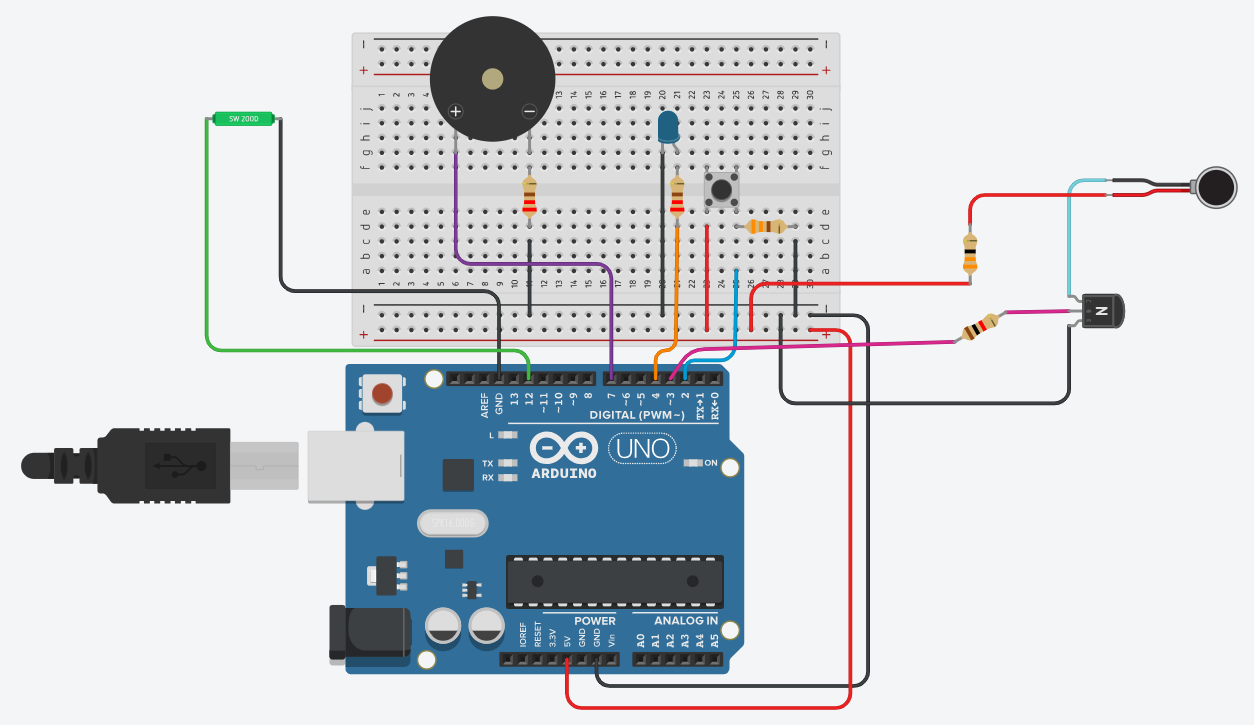
\includegraphics[width=0.8\textwidth]{img/PrototipoV1_Tilt.png}
    \caption{Diagrama de la primera versión del prototipo, empleando el sensor SW520D}
    \label{fig:ProtV1} % Esta etiqueta es la que permite que se encuentr referenciada en el texto (es muy importante que siempre estén referenciadas en el texto)
\end{figure}

\begin{figure}[h]
    \centering
    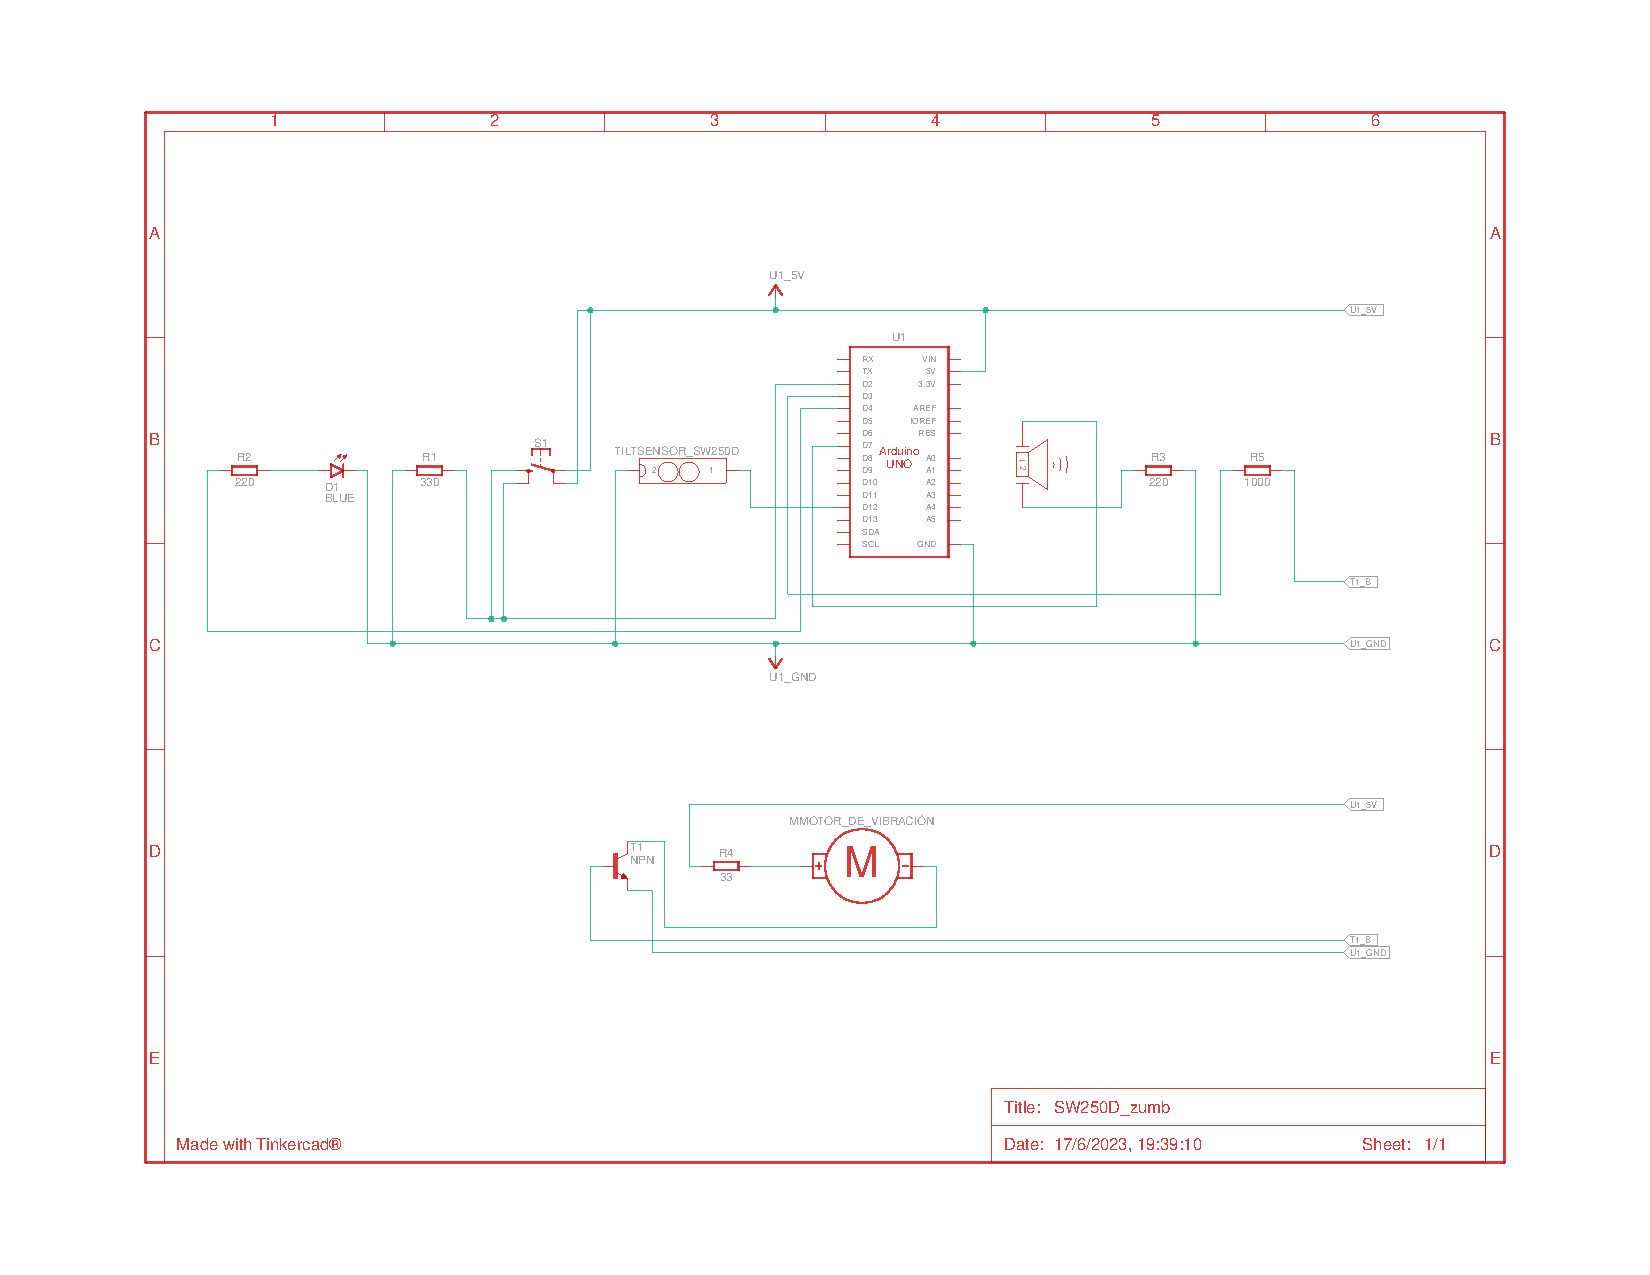
\includegraphics[width=0.9\textwidth]{img/Prot_V1_Esquema.pdf}
    \caption{Diagrama de las realizadas para la implementación de la primera versión del protoripo.}
    \label{fig:ProtV1_esquema} % Esta etiqueta es la que permite que se encuentr referenciada en el texto (es muy importante que siempre estén referenciadas en el texto)
\end{figure}



\newpage
El código empleado para el funcionamiento de esta primera versión ha sido el siguiente:
\begin{lstlisting}
// Led simple + Boton + Zumbador + Tilt + Motor Vibracion
// Naiara Gadea Rodriguez Gomez
// 

int led = 4; // Seleccion del pin del led (pin digital)
int  boton = 2; // Seleccion del pin del boton (pin digital)
int zum = 7;// Seleccion del pin del zumbador
int tilt = 12;// Seleccion del pin del sensor SW250D
int motor = 3; //Seleccion del pin del motor de vibracion

int estado; // Estado del boton

void setup() {
  // put your setup code here, to run once:
  Serial.begin(9600);
  pinMode(led, OUTPUT); // inicializacion del pin led.
  pinMode(boton, INPUT); // inicializacion del pin del boton.
  pinMode(zum, OUTPUT); // inicializacion del pin del zumbador
  pinMode(tilt, INPUT); // inicializacion del pin del sensor tilt
  digitalWrite(tilt , HIGH); // Sensor tilt 
  pinMode(motor, OUTPUT);// inicializacion del pin del motor de vibracion.
}

void loop() {
  // put your main code here, to run repeatedly:
  Serial.println(digitalRead(tilt));// Comprobar en el Serial Monitor.
  if (estado == LOW && digitalRead(boton)){
    // Si se presiona el boton se enciende el dispositivo
    digitalWrite(led, HIGH); // Encendido
      delay(1000); // Durante 1 segundo (1000 ms)
      estado = HIGH; // Cambia el estado del boton a encendido.
    
  }
  if(estado == HIGH){
    // Si el sensor tilt hace contacto, el usuario tiene una mala postura y el dispositivo manda un aviso, musical o de vibracion.
    if (digitalRead(tilt))  {
      // Vibración intermitente
      digitalWrite(motor, HIGH); //vibracion
      delay(500);  // delay 0.5 seconds
      //digitalWrite(motor, LOW);  //stop vibrating
      //delay(500); //wait 0.5 seconds.
      // si vemos que durante la musica no se enciende el motor
      
      melodia(); // En este caso es un aviso sonoro, pero teniendo un motor de vibracion se puede utilizar un aviso vibratorio.
      
    }  else  {
      // Si no hay contacto con el sensor tilt, no suena la melodia
      noTone(zum); // El zumbador ya no emite ruido
      //delay(3000);
      digitalWrite(motor, LOW);// Paramos el motor
    }

    // Si se presiona el boton se apaga el dispositivo
    if (digitalRead(boton)){
      digitalWrite(led, LOW); // Apagado
      delay(1000); // Durante 1 segundo (1000ms)
      estado = LOW; // Cambia el estado del boton a apagado.
    }
    
  }

}

// Definimos las notas
int Do = 261;
int Re = 293;
int Mi = 329;
int Fa = 349;
int Sol = 392;
int La = 440;
int Si = 493;

void melodia(){
  // Escala de musica con el zumbador
    tone(zum, Fa, 500);
    delay(700);
    tone(zum, Sol, 500);
    delay(700);
    tone(zum, Sol, 500);
    delay(700);
    tone(zum, La, 1000);
    delay(1700);
    tone(zum, Sol, 500);
    delay(700);
    tone(zum, Fa, 500);
    delay(700);
    tone(zum, Sol, 500);
    delay(700);
    //tone(zum, Do, 1000);
    //delay(1700);
    //tone(zum, Fa, 500);
    //delay(700);
    //tone(zum, La, 500);
    //delay(700);
    //tone(zum, Fa, 500);
    //delay(700);
    //tone(zum, Re, 1000);
    //delay(1700);
    
}

\end{lstlisting}

Esta versión proporciona un resultado medianamente satisfactorio, porque realiza su función correctamente, pero, puede dar lugar a errores si la persona realiza una inclinación rápida o si el sensor SW520D no está correctamente orientdao. Además esta priemra versión será muy sensible a vibraciones debido a las propias características del sensor empleado.

\subsection{Versión 2, empleando el sensor MPU-6050}

La segunda versiñon se ha creado  en base al microprocesador arduino y el módulo MPU6050.

Esta segunda versión mantiene el botón de encendido, el led de color azul que indica el estado del dispositivo, el zumbador pasivo y el motor de vibración que realizarán el feedback a través de un aviso sonoro o vibratorio.

Además, esta versión cuenta con un botón de calibración para mayor precisión. Este botón deberá presionarse cuando el dispositivo se encienda cuando se coloque por primera vez en la espalda del usuario con una postura correta o en el caso de que el usuario sea consciente de que el dispositivo no esté funcionando correctamente.  

El sensor detecta que la persona se ha inclinado más de 15º de su posición , se detecta una mala postura y se ofrece el feedback sonoro (melodía modificable empleando el zumbador) y vibratorio (motor de vibración) para que el usuario modifique su postura, una vez la persona recupera su postura normal correcta el dispositivo deja de sonar y vibrar, indicando que se encuentra en una postura correcta. Inicialmente se ha creado un umbral de 15º, pero se trata de un umbral modificable.

Se pueden observar los componenetes y las conexiones realizadas en las siguientes imágenes:

\begin{figure}[h!]
    \centering
    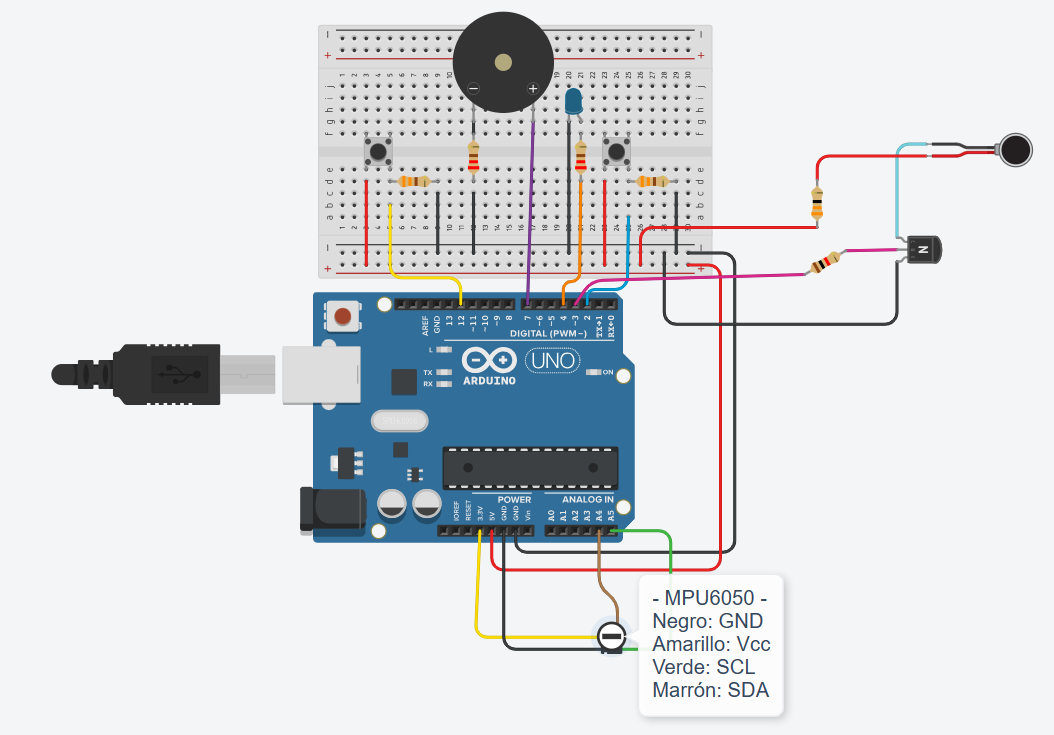
\includegraphics[width=0.8\textwidth]{img/PrototipoV2_MPU6050.png}
    \caption{Diagrama de la segunda versión del prototipo, empleando el módulo MPU-6050}
    \label{fig:ProtV1} % Esta etiqueta es la que permite que se encuentr referenciada en el texto (es muy importante que siempre estén referenciadas en el texto)
\end{figure}

\begin{figure}[h]
    \centering
    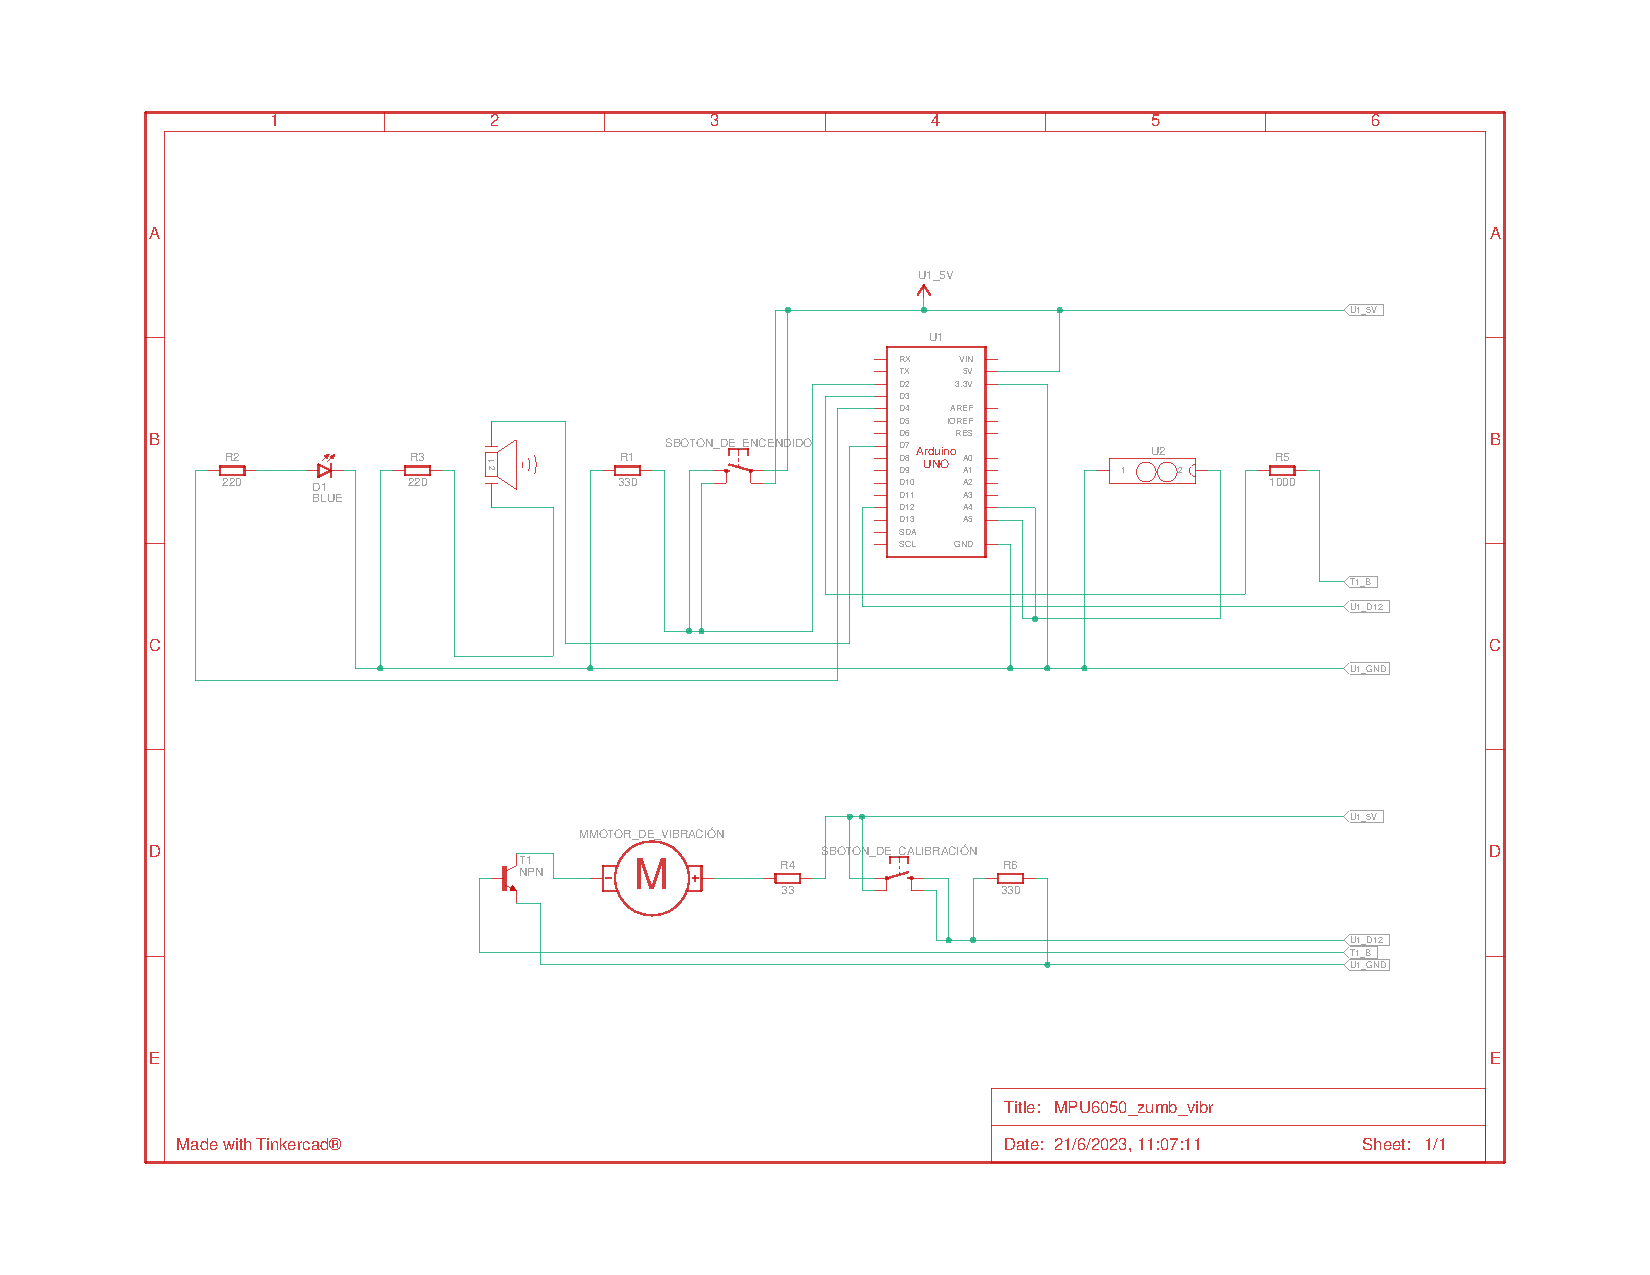
\includegraphics[width=0.9\textwidth]{img/Prot_V2_Esquema.pdf}
    \caption{Diagrama de las conexiones realizadas para la implementación de la segunda versión, siendo el módulo MPU-6050, U2.}
    \label{fig:ProtV1_esquema} % Esta etiqueta es la que permite que se encuentr referenciada en el texto (es muy importante que siempre estén referenciadas en el texto)
\end{figure}



\newpage
El código empleado para el funcionamiento de esta segunda versión es el siguiente:
\begin{lstlisting}
// Led simple + Boton + Zumbador + motor + MPU6050
// Naiara Gadea Rodriguez Gomez
// 

// Librerias I2C para controlar el mpu6050 
// las librerias MPU6050.h, I2Cdev.h y Wire.h 
#include "I2Cdev.h" 
#include "MPU6050.h" 
#include "Wire.h" 

// La direccion del MPU6050 puede ser 0x68 o 0x69, dependiendo  
// del estado de AD0. Si no se especifica, 0x68 estara implicito 

// Se crea la variable del sensor. En este caso se esta trabajando con 0x68. Si se quiere trabajar con 0x69 hay que poner MPU6050 sensor(0x69) 
MPU6050 sensor(0x68); 

// Valores RAW (sin procesar) del acelerometro y giroscopio en los ejes x,y,z 
int ax, ay, az; // acelerometro 
int gx, gy, gz; // giroscopio 

float accel_ang_x, accel_ang_y, accel_ang_z; // Variables correspondientes a los angulos de inclinacion. Son los que nos interesan principalmente.

int  boton1 = 2; // Seleccion del pin del boton (pin digital)
int estado1; // Estado del boton ON/OFF
int led = 4; // Seleccion del pin del led (pin digital)
int zum = 7;// Seleccion del pin del zumbador
int motor = 3; //Seleccion del pin del motor -Cuando se tenga el motor-
int boton2 = 12; //Boton de calibrado
int estado2;//Estado del boton de calibrado

// Otras variables
bool calibrar = false; // Variable que indica cuando seguir o no calibrando.
bool origen = true; // Para guardar los datos del primer valor tras la calibracion.

//Variables usadas por el filtro pasa bajos 
long f_ax,f_ay, f_az; 
int p_ax, p_ay, p_az; 
long f_gx,f_gy, f_gz; 
int p_gx, p_gy, p_gz; 
int counter=0;

//Valor de los offsets 
int ax_o,ay_o,az_o; 
int gx_o,gy_o,gz_o; 

float first_x, first_y, first_z; // Si no funciona correctamente desde el principio, hay que calibrar, o inicializar desde el principio.

float sum_ax, sum_ay, sum_az;
float sum_gx, sum_gy, sum_gz;
float media_ax, media_ay, media_az;
float media_gx, media_gy, media_gz;
int cont = 0;


void setup() {
  // put your setup code here, to run once:
  Serial.begin(9600);
  pinMode(led, OUTPUT); // inicializacion del pin digital led.
  pinMode(boton1, INPUT); // inicializacion del pin digital del boton.
  pinMode(boton2,INPUT); // init del pin boton de calibrado.
  pinMode(zum, OUTPUT); // inicializacion del pin digital del zumbador
  pinMode(motor, OUTPUT);// inicializacion del pin digital del motor de vibracion

  Wire.begin(); //Iniciando I2C   
  sensor.initialize(); //Iniciando el sensor 

  // Al inicializar el sensor los rangos seran: 
  // Acelerometro: -2g a +2g 
  // Giroscopio: -250deg/sec a +250deg/sec 

  // Se comprueba que se ha inicializado correctamente.   
  if (sensor.testConnection()) Serial.println("Sensor iniciado correctamente"); 
  else Serial.println("Error al iniciar el sensor"); 

  // Leer los offset los offsets anteriores (iniciales)
  ax_o=sensor.getXAccelOffset(); 
  ay_o=sensor.getYAccelOffset(); 
  az_o=sensor.getZAccelOffset(); 
  gx_o=sensor.getXGyroOffset(); 
  gy_o=sensor.getYGyroOffset(); 
  gz_o=sensor.getZGyroOffset(); 
  
  Serial.println("Offsets Originales:"); 
  Serial.print(ax_o); Serial.print("\t");  
  Serial.print(ay_o); Serial.print("\t");  
  Serial.print(az_o); Serial.print("\t");  
  Serial.print(gx_o); Serial.print("\t");  
  Serial.print(gy_o); Serial.print("\t"); 
  Serial.print(gz_o); Serial.println("\t"); 
}

void loop() {
  // put your main code here, to run repeatedly:

  if (estado1 == LOW && digitalRead(boton1)){
    // Si se presiona el boton se ENCIENDE EL DISPOSITIVO
    digitalWrite(led, HIGH); // Encendido
      delay(1000); // Durante 1 segundo (1000 ms)
      estado1 = HIGH; // Cambia el estado del boton a encendido.
    
  }
  if(estado1 == HIGH){
    // Si el sensor tilt hace contacto, el usuario tiene una mala postura y el dispositivo manda un aviso, musical o de vibracion.
    
    // Leer las aceleraciones y velocidades angulares y se guardan en sus variables 
    sensor.getAcceleration(&ax, &ay, &az); 
    sensor.getRotation(&gx, &gy, &gz);

    if (digitalRead(boton2) && estado2==LOW){
      calibrar = true;
    }

    if (calibrar){
      //Serial.println("Se ha dado el boton, calibrar"); 
      calibracion();
      origen = true;
    }else{
      if(origen){
        first_x=accel_ang_x;
        first_y = accel_ang_y;
        first_z = accel_ang_z;

        origen = false;
      }

      if (cont < 10){
        lecturas();
        sum_ax = sum_ax + accel_ang_x; // queremos el angulo de inclinacion.
        sum_ay = sum_ay + accel_ang_y; // queremos el angulo de inclinacion.
        sum_az = sum_az + accel_ang_z; // queremos el angulo de inclinacion.

        cont++;

      } else{
        media_ax = sum_ax/10;
        Serial.print("Valor medio de inclinacion en X cada 5 s: "); Serial.println(media_ax);
        media_ay = sum_ay/10;
        Serial.print("Valor medio de inclinacion en Y cada 5 s: "); Serial.println(media_ay);
        media_az = sum_az/10;
        Serial.print("Valor medio de inclinacion en Z cada 5 s: "); Serial.println(media_az);
        // reestablecemos los sumatorios
        sum_ax = 0; 
        sum_ay = 0; 
        sum_az = 0; 
        cont = 0;

        if(abs(first_x - media_ax)<15 & abs(first_y - media_ay)<15 & abs(first_z - media_az)<15){
          Serial.println("Buena postura");
          noTone(zum); // NO se produce alerta
          digitalWrite(motor, LOW);// Paramos el motor -Cuando se tenga motor.
        }else{
          Serial.println("Mala postura, ponte recto");
          digitalWrite(motor, HIGH); //vibracion -Cuando se tenga motor.
          //delay(500);  // delay one second -Cuando se tenga motor.
          melodia(); // Se produce alerta
          
        }

      }

    } 

    // Si se presiona el boton se apaga el dispositivo
    if (digitalRead(boton1)){
      digitalWrite(led, LOW); // Apagado
      delay(1000); // Durante 1 segundo (1000ms)
      estado1 = LOW; // Cambia el estado del boton a apagado.
    }
    
  }

}

void lecturas(){
  // Si queremos pasar las lecturas del acelerometro a m/s^2 hay que multiplicar las lecturas por (9.81/16384.0). 
  // En la componente Z se deben encontrar mediciones aproximadas a los 9.8 m/s^2 
  // Si queremos pasar las lecturas del giroscopio a deg/s (grados/s) hay que multiplicar las lecturas por (250.0/32768.0) 
  //Mostrar las lecturas separadas por un [tab] 
  Serial.print("a[x y z]   Incl X   Incl Y  g[x y z]:\t"); 
  Serial.print(ax*(9.81/16384.0)); Serial.print("\t"); // En m/s^2
  Serial.print(ay*(9.81/16384.0)); Serial.print("\t"); // En m/s^2
  Serial.print(az*(9.81/16384.0)); Serial.print("\t"); // En m/s^2

  accel_ang_x=atan(ax/sqrt(pow(ay,2) + pow(az,2)))*(180.0/3.14); // En angulos de inclinacion
  Serial.print(accel_ang_x); Serial.print("\t"); 
  accel_ang_y=atan(ay/sqrt(pow(ax,2) + pow(az,2)))*(180.0/3.14); // En angulos de inclinacion
  Serial.print(accel_ang_y); Serial.print("\t"); 
  accel_ang_z=atan(az/sqrt(pow(ax,2) + pow(ay,2)))*(180.0/3.14); // En angulos de inclinacion
  Serial.print(accel_ang_z); Serial.print("\t"); 
  
  // Esto no es necesario
  Serial.print(gx*(250.0/32768.0)); Serial.print("\t"); // En grados/s
  Serial.print(gy*(250.0/32768.0)); Serial.print("\t"); // En grados/s 
  Serial.println(gz*(250.0/32768.0)); // En grados/s

  delay(500); // Mide cada 0,5 segundos, la media para comprobar que se encuentra en una buena postura sera cada 10 medidas (cada 5 segundos)

}

void calibracion(){
  // Filtrar las lecturas 
  f_ax = f_ax-(f_ax>>5)+ax; 
  p_ax = f_ax>>5; 

  f_ay = f_ay-(f_ay>>5)+ay; 
  p_ay = f_ay>>5; 

  f_az = f_az-(f_az>>5)+az; 
  p_az = f_az>>5; 

  f_gx = f_gx-(f_gx>>3)+gx; 
  p_gx = f_gx>>3; 

  f_gy = f_gy-(f_gy>>3)+gy; 
  p_gy = f_gy>>3; 

  f_gz = f_gz-(f_gz>>3)+gz; 
  p_gz = f_gz>>3; 
  
  //Cada 100 lecturas corregir el offset 
  if (counter==100){ 
    //Serial.print("Calibrando...");
    //Mostrar las lecturas separadas por un [tab] 
    Serial.print("promedio:"); Serial.print("\t"); 
    Serial.print(p_ax); Serial.print("\t"); 
    Serial.print(p_ay); Serial.print("\t"); 
    Serial.print(p_az); Serial.print("\t"); 
    Serial.print(p_gx); Serial.print("\t"); 
    Serial.print(p_gy); Serial.print("\t"); 
    Serial.println(p_gz); 
    //Basicamente, se modifica constantemente el offset para que sea 0, como medida real. 
    // Una vez se observen valores cercanos a 0 se debe desconectar o reiniciar el Arduino, y asi ya se encuentra calibrado el dispositivo. 
    //Calibrar el acelerometro a 1g en el eje z (ajustar el offset) 
    if (p_ax>0) ax_o--; 
    else {ax_o++;} 
    
    if (p_ay>0) ay_o--; 
    else {ay_o++;} 
    
    if (p_az-16384>0) az_o--; 
    else {az_o++;} 
    
    sensor.setXAccelOffset(ax_o); 
    sensor.setYAccelOffset(ay_o); 
    sensor.setZAccelOffset(az_o); 
    
    //Calibrar el giroscopio a 0deg/s en todos los ejes (ajustar el offset) 
    if (p_gx>0) gx_o--; 
    else {gx_o++;} 
    
    if (p_gy>0) gy_o--; 
    else {gy_o++;} 
    
    if (p_gz>0) gz_o--; 
    else {gz_o++;} 

    sensor.setXGyroOffset(gx_o); 
    sensor.setYGyroOffset(gy_o); 
    sensor.setZGyroOffset(gz_o);
    
    counter=0; 

    if (p_ax>-10 & p_ax<10 & p_ay>-10 & p_ay<10 & p_az>16374 & p_az<16394 & p_gx>-10 & p_gx<10 & p_gy>-10 & p_gy<10 & p_gz>-10 & p_gz<10){
      Serial.println("DISPOSITIVO CALIBRADO!!!");
      calibrar = false;
    }else{
      Serial.println("Calibrando...");
    }
  } 
  counter++;

}


// Definimos las notas
int Do = 261;
int Re = 293;
int Mi = 329;
int Fa = 349;
int Sol = 392;
int La = 440;
int Si = 493;

void melodia(){
  // Escala de musica con el zumbador
    tone(zum, Fa, 500);
    delay(700);
    tone(zum, Sol, 500);
    delay(700);
    
}


\end{lstlisting}

Esta versión proporciona un resultado satisfactorio, porque realiza su función correctamente, aunque hay que calibrarlo cada vez que se enciende el dispositivo y la calibración puede llevar varios minutos. Además, habría que modificar el ángulo de aviso que se quiere tener de umbral de correcta o incorrecta postura. También se puede modificar el tiempo de espera que se quiere tener para dar el aviso de una postura incorrecta, en este caso se encuentra a 5 segundos.

Por otro lado, hay que pensar en cómo posicionar de forma correcta el dispositivo con el sensor en la espalda del usuario, ya que el sensor debe estar en horizontal. Si no se coloca correctamente el sensor habría que modificar los ejes en el código, ya que no detectara de forma correcta los ángulos y esto puede ser algo complejo.

%%%%%%%%%%%%%%%%%%%%%%%%%%%%%%%%%%%%%%%
\newpage
\section{Manuales y/o Demostraciones prácticas}[h!]

Introducir XXXXXXXXXXXXXXXXXXXXXXXXXXXXXXXXx

Incluir imágenes de cada paso al utilizar cada una de las versiones.




    
     